\documentclass[11pt]{article}
\usepackage{array, xcolor}
\usepackage[margin=1.5cm]{geometry}
\usepackage{hyperref}

\usepackage{graphicx,mwe}
\usepackage{array}
\usepackage{graphicx}
\usepackage{wrapfig}

\usepackage{enumitem}

\usepackage{fontspec}
\setmainfont{Helvetica}
\setsansfont{DejaVu Sans}
\setmonofont{DejaVu Sans Mono}
\usepackage{fontsize}
\changefontsize[13]{12}

\usepackage[none]{hyphenat}

\title{\bfseries\Huge Oleg Shpynov}
\author{\textbf{oleg.shpynov@gmail.com}}
\date{}

\definecolor{lightgray}{gray}{0.8}
\newcolumntype{L}{>{\raggedleft}p{0.16\textwidth}}
\newcolumntype{R}{p{0.8\textwidth}}
\newcommand\VRule{\color{lightgray}\vrule width 0.5pt}

%%% Begin Document
\begin{document}
	\maketitle 
	
	\begin{wrapfigure}{r}{0.4\textwidth}
		\vspace*{-4cm} % moving actual picture up
		\hfill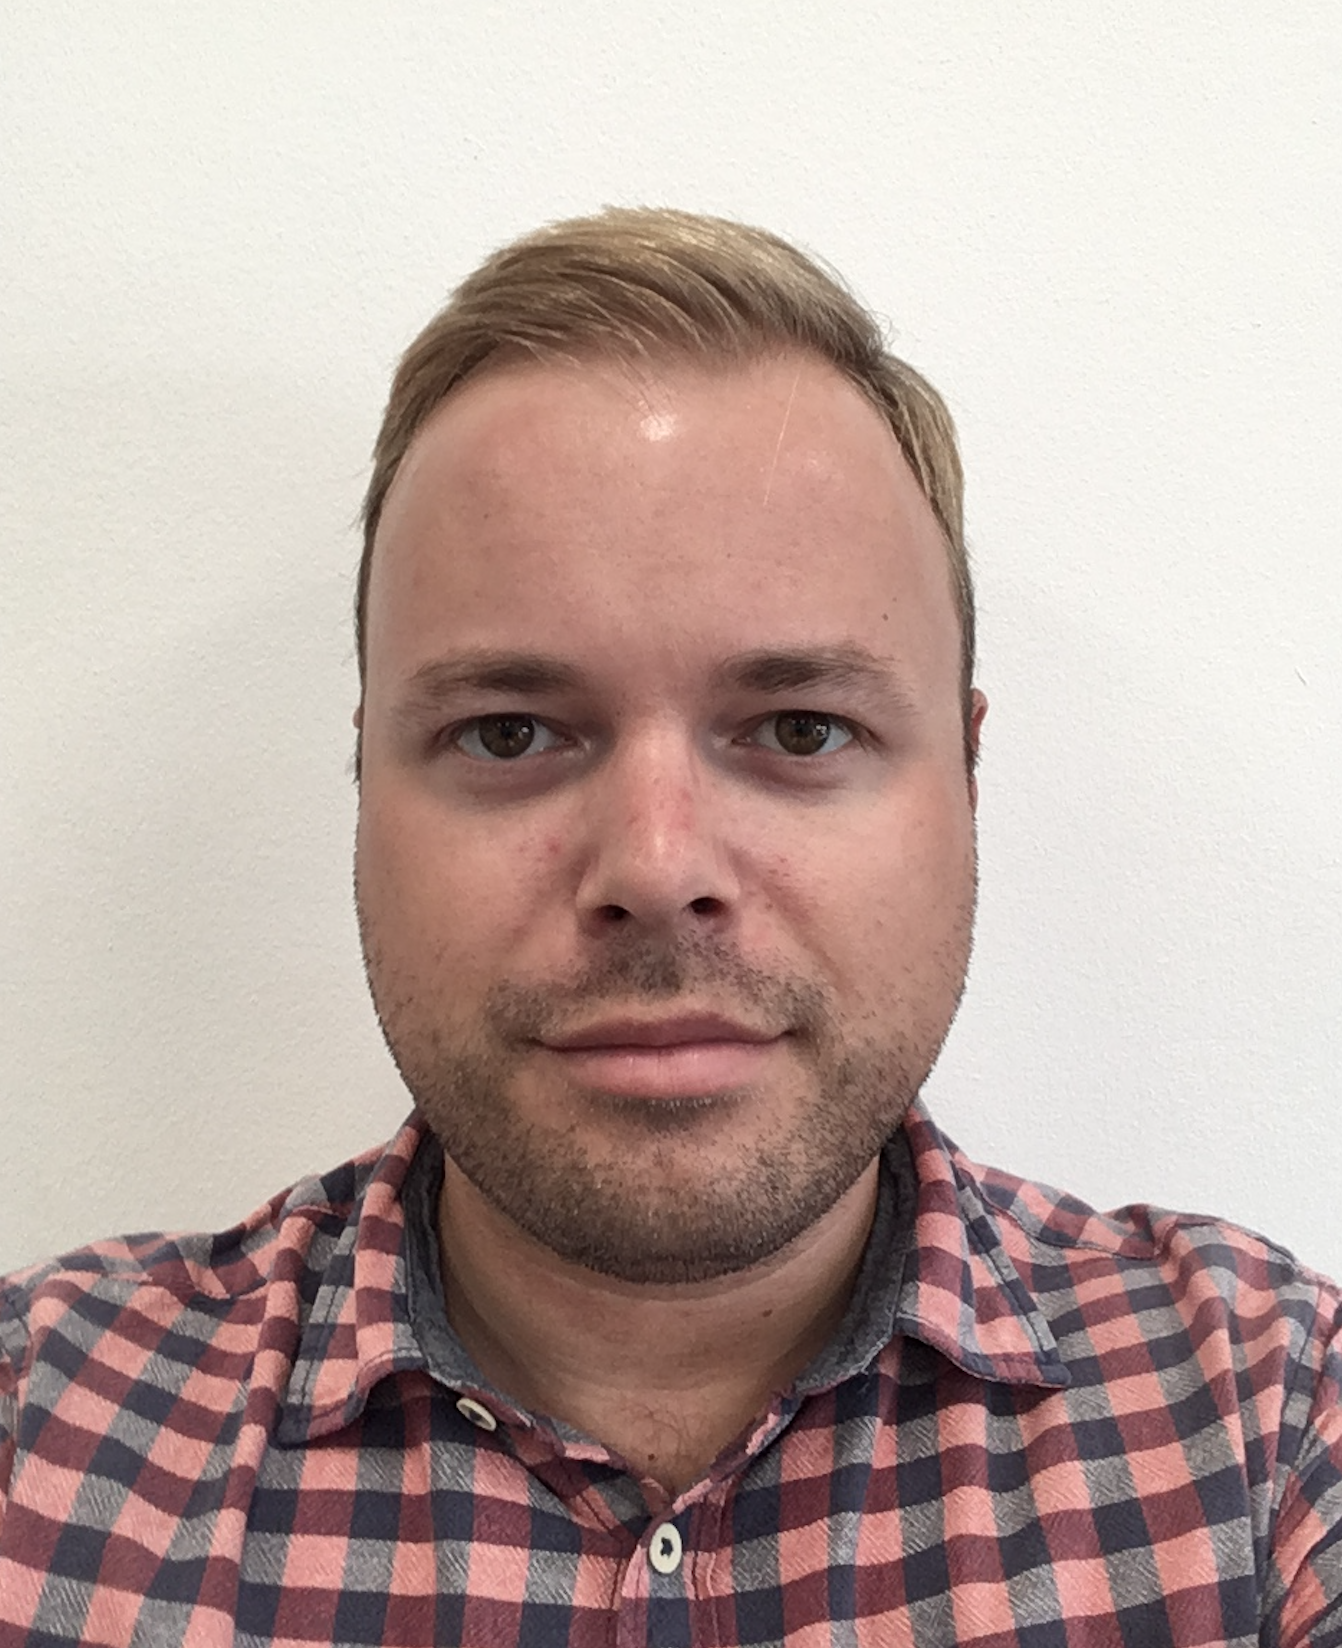
\includegraphics[width=0.20\textwidth]{me2020.png}
		\vspace*{-4cm} % avoid real text wrapping
	\end{wrapfigure}
	
	
	
	%%% Personal details
	\hspace*{-0.6cm}\begin{minipage}[ht]{0.4\textwidth}
		80999 Waltenbergerstr. 11\\
		Munich, Germany
	\end{minipage}
	\begin{minipage}[ht]{0.4\textwidth}
		April 7th, 1986\\
		+ 49 177 6904790
	\end{minipage}
	\vspace{10pt}

%%% About me short
\section*{Summary}
Seasoned research and development engineering leader with strong math background, good \\
communication and teamwork skills. I am leading a group that develops machine learning algorithms, bioinformatics software and scalable computational  pipelines for data analysis. Took part in the development of major JetBrains products with focus on the code analysis from lexical analysis to advanced type system development and semantic verifications.
%%% Professional experience
\section*{Experience}
\begin{tabular}{L!{\VRule}R}
2014 -- today & \textbf{Research and Development Team Lead}\\
& \textit{JetBrains Research, Munich, Germany}\\[5pt]
& Head of research and development group. Group is developing novel algorithms and methods for experimental data analysis, building scalable computational pipelines and tools, and working in collaboration with researchers on various bionformatics studies.\\
& \setlist{nolistsep}

\begin{itemize}[noitemsep]
	\item Built a team of software developers with expertise in software development, machine learning, data analysis and bioinformatics
	\item Lead development of two products: \href{https://github.com/JetBrains-Research/jbr}{JBR Genome Browser} and \href{https://github.com/JetBrains-Research/span}{SPAN Semi-supervised Peak Analyzer}
	\item Developed various open source libraries including Viktor (vector computations for Kotlin), Bioinf-commons (Bioinformatics library in Koltin), big (BigBed/Wig files format support for JVM), npy (Numpy arrays support for JVM)
	\item Developed web application for scientific papers analysis \href{https://github.com/JetBrains-Research/pubtrends}{PubTrends}
	\item Authored scientific papers
	\item Onboarding and mentoring software developers of all levels
	\item Coordinated research and development activities

\end{itemize}\\
& Applied technologies: Unix, Java, Kotlin, Swing, Python, Jupyter, Pandas, Matplotlib, Docker, Docker Compose, PostgreSQL, Neo4j, Flask, Celery, Nltk, Pytorch, HTML, CSS, Javascript, React, Bootstrap, Git, GitHub, AWS, Continuous Integration TeamCity\\[5pt]
& Group website: \href{https://research.jetbrains.org/groups/biolabs}{https://research.jetbrains.org/groups/biolabs}\\
& Personal GitHub account: \href{https://github.com/olegs}{https://github.com/olegs}\\
\end{tabular}

\begin{tabular}{L!{\VRule}R}

2014 -- today  & \textbf{Students Mentor}\\
& \textit{Computer Science Center, Saint-Petersburg, Russia}\\
& \textit{Higher School of Economics, Saint-Petersburg, Russia}\\
& \textit{Bioinformatics Institute, Saint-Petersburg, Russia}\\[5pt]
& Mentored various student project in software development and machine learning including two successful Masters dissertations\\
& \\
2006 -- 2013 & \textbf{Senior Software Developer}\\
& \textit{JetBrains, Saint-Petersburg, Russia}\\[5pt]
& Main focus was on the analysis of source code in programming languages, starting from lexical analysis to advanced type system development and source code semantic verifications.  Developed from scratch the most intelligent IDE for Ruby and Rails - RubyMide IDE, language and frameworks support.\\


& \setlist{nolistsep}
\begin{itemize}[noitemsep]
	\item Developed JetBrains products: flagship tool \href{https://jetbrains.com/idea}{IntellIJ IDEA}, \href{https://jetbrains.com/pycharm}{PyCharm}
	\item Created \href{http://jetbrains.com/ruby}{RubyMine} IDE for Ruby programming language	
	\item Maintained and developed \href{https://plugins.jetbrains.com/plugin/164?pr=idea}{IdeaVIM} plugin (vim emulation plugin, 7+mln downloads)
	\item Various plugins development including GitHub integration support, web-markup languages editing capabilities like YAML, SCSS, LESS, etc.
	\item Participated in conferences on Ruby on Rails as a speaker
	\item Authored \href{https://blog.jetbrains.com/ruby/author/oleg_s/}{blog} blogposts on Rubymine, IntelliJ IDEA, etc.
\end{itemize}\\
& Applied technologies: Ruby, Rails, Unix, Java, Concurrency, IDE, Swing, Git, GitHub, Continuous Integration TeamCity\\[5pt]
& Website: \href{https://www.jetbrains.com}{https://www.jetbrains.com/}\\

\end{tabular}


%%% Education
\section*{Education}
\begin{tabular}{L!{\VRule}R}
2020 & Product management course by Computer Science Center, Saint-Petersburg\\
& Product management, startup enterpreneurship \\ 
& \\

2019 & Deep learning nanodegree at Udacity, certificate number: 9GSNRHUA  \\
& Machine learning, deep learning, models deployment \\ 
& \\
2015 & Microsoft Machine Learning and Intelligence School, Microsoft, Russia \\
& Machine learning, artificial intelligence, statistics. \\ 
& \\
2011 -- 2012 & Saint-Petersburg Academic University — Nanotechnology Research and Education Centre of the Russian Academy of Sciences, Russia\\
& Bioinformatics, molecular biology, statistics. \\
& \\
2003 -- 2008 & Masters in Computer Science, Diploma with honors, score 4.9 of 5. \\
& Saint-Petersburg State University, Russia \\
& Faculty of Mathematics and Mechanics, Department of System Programming \\
\end{tabular}
 
\section*{Publications}
\begin{tabular}{L!{\VRule}R}
2021 & \textbf{Oleg Shpynov}, Kapralov Nikolai; "PubTrends: a scientific literature explorer", BCB '21: Proceedings of the 12th ACM Conference on Bioinformatics, Computational Biology, and Health Informatics, Article No.: 72, Pages 1 \\

& \href{https://dl.acm.org/doi/10.1145/3459930.3469501}{DOI 10.1145/3459930.3469501}\\
&\\
2021 & \textbf{Oleg Shpynov}, Aleksei Dievskii, Roman Chernyatchik, Petr Tsurinov, Maxim N Artyomov; "Semi-supervised peak calling with SPAN and JBR Genome Browser", Bioinformatics, Volume 37, Issue 22, 15 November 2021, Pages 4235–4237\\
& \href{https://doi.org/10.1093/bioinformatics/btab376}{DOI 10.1093/bioinformatics/btab376}\\
&\\
2020 & Anna Nikiforovskaya, Nikolai Kapralov, Anna Vlasova, \textbf{Oleg Shpynov}, Aleksei Shpilman; "Automatic generation of reviews of scientific papers, 2020 19th IEEE International Conference on Machine Learning and Applications (ICMLA)\\
& \href{https://doi.org/10.1109/ICMLA51294.2020.00058}{DOI 10.1109/ICMLA51294.2020.00058}\\
\end{tabular}

\section*{Languages}
\begin{tabular}{L!{\VRule}R}
Russian & Native\\
English & Fluent\\
German & Elementary
\end{tabular}

\section*{Honors and Awards}
\begin{tabular}{L R}
& ACM ICPC programming contests participant in University Team \\
&  Winner of Saint-Petersburg State school contests on Mathematics, Physics, Programming
\end{tabular}

\section*{Interests}
\begin{tabular}{L R}
	& Machine learning, data analysis, and bioinformatics.
	\\
	& Traveling, hiking, snowboarding, diving, cycling, photography. \\
\end{tabular}
 
\end{document}